%%% Kapitel "uber Erweiterung der EFA auf periodische St"orungen
%   Time-stamp: <1999-03-04 11:28:40 ralf>

%%%%%%%%%%%%%%%%%%%%%%%%%%%%%%%%%%%%%%%%%%%%%%%%%%%%%%%%%%%%%%%%%%%%%%%
%%%%%%%%%%%%%%%%%%%%%%%%%%%%%%%%%%%%%%%%%%%%%%%%%%%%%%%%%%%%%%%%%%%%%%%
%%%
%%%[Periodische St"orungen mit \kdotp]
\chapter{Periodische St"orungen im Rahmen der \kdotp-Theorie}
\label{cha:period-stoer}

In diesem Kapitel soll die allgemeine Theorie f"ur die Verallgemeinerung der
\kdotp-Theorie auf periodische St"orungen vorgestellt werden. Dazu wollen wir
zun"achst die Standard \kdotp-Theorie skizzieren, wie sie etwa bei Kane
\cite{kane:66} zu finden ist, und danach die n"otigen Verallgemeinerungen
vornehmen. 

%%%%%%%%%%%%%%%%%%%%%%%%%%%%%%%%%%
\section{Standard \kdotp-Theorie}
\label{sec:standard-k.p}

Im Rahmen der \kdotp-Theorie wird normalerweise das Problem eines Elektrons in
einem periodischen Potential behandelt, d.~h.\ die station"are
Schr"odinger-Gleichung mit dem Hamilton-Operator
%
\begin{displaymath}
  \op{H_{0}} = \frac{\vecop{p}^{2}}{2m} + \op{V_{0}}(\vecop{r}).
\end{displaymath}
%
Dabei ist \vecop{p} der Impulsoperator, $\op{V_{0}}(\vecop{r})$ das
ortsabh"angige Kristallpotential und $m$ die Masse des freien Elektrons.
Gesucht sind dann die Eigenfunktionen $\psi_{n}$ und Energieeigenwerte
$\veps_{n}$ des Eigenwertproblems 
%
\begin{equation}
  \label{eq:standard-SG}
  \op{H_{0}} \psi_{n} =  \left[ \frac{\vecop{p}^{2}}{2m} +
  \op{V_{0}}(\vecop{r}) \right] \psi_{n} = \veps_{n} \psi_{n} .
\end{equation}
%
Das Bloch-Theorem besagt, da"s sich $\psi_{n}$ als
%
\begin{equation}
  \label{eq:bloch}
  \psi_{n} \equiv  \psi_{n\ak}(\vec{r}) = e^{i\sprod{\ak}{r}}
  u_{n\ak}(\vec{r}) 
\end{equation}
%
schreiben l"a"st, wobei $u_{n\ak}(\vec{r})$ die selbe Periodizit"at wie
$\op{V_{0}}(\vecop{r})$ hat und \ak\ ein Wellenvektor aus der ersten
Brillouin-Zone ist. Betrachten wir die Zust"ande mit verschiedenem Bandindex
$n$ aber \emph{einem} $\ak_{0}$ aus der ersten Brillouin-Zone, so bilden sie
eine vollst"andige Basis. Luttinger und Kohn \cite{luko:55} haben gezeigt,
da"s auch 
%
\begin{equation}
  \label{eq:altebasis}
  \altebasis = e^{i\sprod{\ak}{r}} e^{i\sprod{\ak_{0}}{r}} u_{n\ak_{0}}(\vec{r})
\end{equation}
%
eine orthonormale und vollst"andige Basis bilden. Wir k"onnen also die
gesuchte L"osung $\psi_{n}$ in die \altebasis\ zu einem $\ak_{0}$ entwickeln
%
\begin{equation}
  \label{eq:standard-entwicklung}
  \psi_{n} = \sum_{\pri{n}} \int \vdx{\akb} c_{n\pri{n}}(\ak) \paltebasis .
\end{equation}

Setzen wir nun die Entwicklung \eqref{eq:standard-entwicklung} in die
station"are Schr"odinger-Glei"-chung \eqref{eq:standard-SG} ein, so stellen wir
fest, da"s sich die Energieeigenwerte $\veps_{n}$ mit dem Wellenvektor \ak\ 
charakterisieren lassen. Dies war auf Grund des Bloch-Theorems auch zu
erwarten, und wir erhalten die bekannte \kdotp-Gleichung
%
\begin{equation}
  \label{eq:standard-k.p}
   \left( \veps_{n}(\ak_{0}) + \frac{\hbar^{2}}{2m}\akb^{2} \right) c_{nn}(\ak)
  + \sum_{\pri{n}} \frac{\hbar}{m} \sprod{\ak}{\pnn} c_{n\pri{n}}(\ak)
  = \veps_{n}(\ak) c_{nn}(\ak)
\end{equation}
%
mit den Impulsmatrixelementen
%
\begin{equation}
  \label{eq:pnn}
  \pnn := {\frac{(2\pi)}{\Omega_{0}}}^{3} \int \vdx{r}
  e^{-i\sprod{\ak_{0}}{r}} \cc{u_{n\ak_{0}}} \, \op{\vec{p}} \,
  e^{i\sprod{\ak_{0}}{r}} u_{\pri{n}\ak_{0}}.
\end{equation}
%
Dabei geht das Integral "uber die Einheitszelle mit Volumen
$\Omega_{0}$.\footnote{Kane \cite{kane:66} definiert die Impulsmatrixelemente
  zwischen den gitterperiodischen Anteilen der Bloch-Zust"ande, Luttinger und
  Kohn \cite{luko:55} zwischen den Bloch-Zust"anden selbst. Wir folgen
  letzterem Beispiel.}

Gl.~\eqref{eq:standard-k.p} ist "aquivalent zur Schr"odinger-Gleichung
\eqref{eq:standard-SG}, von der wir ausgegangen sind. Um nun
Gl.~\eqref{eq:standard-k.p} zu l"osen, ben"otigen wir alle Eigenenergie
$\veps_{n}(\ak_{0})$ am Entwicklungspunkt $\ak_{0}$, sowie alle
Impulsmatrixelemente \pnn\ zwischen diesen Zust"anden. Wir haben es dabei aber
mit einem unendlich-dimensionalen Gleichungssystem zu tun, weshalb
normalerweise Gl.~\eqref{eq:standard-k.p} f"ur kleine Werte von \akb\ 
st"orungstheoretisch behandelt wird. Das bekannteste Ergebnis solch
einer Rechnung, die Gleichung f"ur die efffektive Masse der Elektronen,
erhalten wir, wenn wir f"ur ein nichtentartetes Band an einem Extremum der
Energiedispersion bis zur zweiten Ordnung in \akb\ entwickeln:
%
\begin{equation}
  \label{eq:standard-m*}
  E(\ak) = \veps_{n}(\ak_{0}) + \frac{\hbar^{2}}{2m}\akb^{2} + 
  \left(\frac{\hbar}{m}\right)^{2} \sum_{\pri{n}}
  \frac{|\sprod{\ak}{\pnn}|^{2}}{\veps_{n}(\ak_{0})-\veps_{\pri{n}}(\ak_{0})}
\end{equation}

Oft reicht es nicht aus, sich wie in Gl.~\eqref{eq:standard-m*} nur auf ein
nichtentartetes Band zu beschr"anken. Eine systematische M"oglichkeit die
au"serdiagonalen St"orungen in Gl.~\eqref{eq:standard-k.p} zu ber"ucksichtigen
bietet die L"owdin St"orungstheorie \cite{lowd:51}.
% Diese erlaubt es, in einer systematischen
%Art und Weise den Einfl"u"s energetisch weit entfernter B"ander auf die
%Zust"ande, die genauer untersucht werden sollen, zu ber"ucksichtigen. 
Dieses Verfahren k"onnen wir uns so vorstellen, da"s die 
Schritte, die normalerweise bei einer (pseudo-)entarten St"orungstheorie in
der Quanten-Mechanik durchgef"uhrt werden m"ussen, in umgekehrter Reihenfolge
durchgef"uhrt werden. Es werden
\emph{zun"achst} die Einfl"usse der energetisch weit entfernten Zust"ande
ber"ucksichtigt und erst dann die verbliebene Matrix f"ur den
(pseudo-)entarteten Unterraum diagonalisiert. Da die Reihenfolge der Schritte
umgekehrt wurde, f"uhrt der erste Schritt auch zu Ver"anderungen in den
Kopplungskonstanten, d.~h.\ in den Ausserdiagonaltermen der verbleibenden
Matrix, die bei normaler (pseudo-)"-entarteter St"orungstheorie nicht
auftreten.

Formal bedeutet dies, da"s die Zust"ande unseres Systems in zwei
Gruppen aufgeteilt werden. Die Zust"ande in Gruppe \raum{A} sind diejenigen,
die uns interessieren und deren Wechselwirkungen wir exakt behandeln wollen.
Die Zust"ande in Gruppe \raum{B} haben nur eine schwache Wechselwirkung mit
denen in \raum{A}. Diese Wechselwirkung wird in St"orungstheorie
ber"ucksichtigt.  Dabei wird die Wechselwirkungsmatrix $H_{i j}$ der Zust"ande
in \raum{A} wie folgt abge"andert:\footnote{Diese bez"uglich der Energienenner
  symmetrische Form ist z.~B.\ bei Bir und Pikus \cite{bipi:74} zu finden.}
%
\begin{displaymath}
%  \label{eq:lowd}
  \tilde{H}_{ij} = H_{ij} + \frac{1}{2} \sum_{\beta \in \raum{B}} H_{i \beta}
  H_{\beta j} \left( \frac{1}{E_{i}-E_{\beta}} + \frac{1}{E_{j}-E_{\beta}}
  \right) + \dots
\end{displaymath}
%
Dadurch erhalten wir ein endliches Gleichungssystem, das es uns erm"oglicht,
die Entwicklungskoeffizienten $c_{n\pri{n}}(\ak)$ mit $n \in \raum{A}$ zu
bestimmen und aus diesen dann die Entwicklungskoeffizienten f"ur $n \in
\raum{B}$ zu erhalten.

Sollen im Rahmen der Standard \kdotp-Theorie Valenzband-Zust"ande beschrieben
werden, so m"ussen wir meist die Spin-Bahn-Wechselwirkung
be"-r"ucksichtigen. Diese f"uhrt zu einem zus"atzlichen Term der Form 
%
\begin{equation}
  \label{eq:Spin-Bahn}
  \op{H_{\text{SO}}} = \frac{\hbar}{4m^{2}c^{2}} (\grvecop{\sigma} \times
  \nabla\op{V}) \cdot \vecop{p}
\end{equation}
%
im Hamilton-Operator. Dabei ist \grvecop{\sigma} der Vektor der
Pauli-Spin-Matrizen und \op{V} das Kristallpotential.

Dieser Term wird normalerweise st"orungstheoretisch so behandelt, da"s er im
Unterraum entarteter Zust"ande diagonalisiert wird. Dadurch erh"oht sich die
Anzahl der notwendigen Parameter nur um die jeweiligen Spin-Bahn-Aufspaltungen
\cite{kane:66}. F"ur die Wechselwirkung mit anderen Zust"anden m"ussen
wir nur von den \pnn\ zu $\grvec{\pi}_{\mathnormal{n\pri{n}}}$
"ubergehen, die sich in ihrer Definition darin unterscheiden, da"s in
Gl.~\eqref{eq:pnn} \vecop{p} durch $\vecop{p} +
\frac{\hbar}{4mc^{2}} (\grvecop{\sigma} \times \nabla\op{V})$ ersetzt
werden mu"s \cite{luko:55}. 

Verzerrungen auf Grund "au"seren Drucks lassen sich mit der
Invarianten-Theorie ber"ucksichtigen, wie sie Bir und Pikus \cite{bipi:74}
entwickelt haben. 

Bei St"orungen, die die Periodizit"at des Kristalls brechen, wie z.~B.\ flache
St"orstellen oder Magnetfelder, k"onnen wir zur Envelopfunktionsn"aherung
(EFA) \cite{luko:55} "ubergehen, und so eine gute Beschreibung der
auftretenden Ph"anomene finden. Die dabei erhaltenen Gleichungen sind nicht
mehr diagonal in \ak. Vielmehr kommt es zu Wechselwirkungen zwischen
Zust"anden in der Umgebung des Entwicklungspunktes $\ak_{0}$.

Wie wir gesehen haben, ist die Standard \kdotp-Theorie auf ein gro"se Anzahl
von Problemen anwendbar, oder aber es bestehen Erweiterungen wie die EFA. Dies
ist nicht der Fall f"ur periodischen und insbesondere kommensurable
St"orungen,\footnote{Ein periodisches St"orpotential hei"st dann kommensurabel
  zum urspr"unglichen Potential, wenn sich dessen primitive Gittervektoren als
  ganzzahlige Linearkombinationen der urspr"unglichen Gittervektoren schreiben
  lassen.}
wie wir sie hier betrachten wollen. 

%%%%%%%%%%%%%%%%%%%%%%%%%%%%%%%%%%%%%%%%%%%%%%%%%%%%%%%%%%%%%%%%%%%%%%%%%
%%%
%%% Wahl der Basis
%%%
\section{Wahl der Basis}
\label{sec:basis}

Zu unserm Gesamtproblem, d.~h.\ ungest"orter Kristall plus periodisches
St"or"-potential, geh"ort eine neue Einheitszelle (nEZ), die gr"o"ser als die 
alte Einheitszelle (aEZ) ist. Auf Grund der Kommensurabilit"at der St"orung,
lassen sich die Basisvektoren zur neuen Einheitszelle als ganzzahlige
Vielfache der alten Basisvektoren schreiben.

Im reziproken Raum drehen sich diese Verh"altnisse um. Die neue
Bril"-louin-Zone (nBZ) ist \emph{kleiner} als die alte Brillouin-Zone (aBZ),
und die alten Basisvektoren im reziproken Raum lassen sich als ganzzahlige
Linearkombination der neuen Basisvektoren darstellen.

Das bedeutet aber, da"s zu den reziproken Gitterpunkten $\{\aG\}$ unseres
ungest"orten Systems neue Vektoren hinzukommen. Unser Gesamtproblem besitzt
also reziproke Gittervektoren $\{\nG\}$, wobei
%die alten reziproken Gitterpunkten 
$\{\aG\}$ eine Teilmenge
%der neuen reziproken Gitterpunkten 
von $\{\nG\}$ ist.

Die neuen reziproken Gittervektoren f"uhren dazu, da"s an jedem Punkt der
neuen Brillouin-Zone Zust"ande zu finden sind, die von verschiedenen Punkten
der alten Brillouin-Zone kommen. Dieser Vorgang ist auch als (R"uck-) Faltung
von Zust"anden bekannt. Diese auf einen Punkt im reziproken Raum
zur"uckgefalteten Zust"ande werden i.~A.\ auch wechselwirken, und die sich
daraus ergebenden Effekte wollen wir untersuchen. Schwierigkeiten mit der
Standard \kdotp-Theorie ergeben sich, weil die r"uckgefalteten Zust"ande aus
der gesamten alten Brillouin-Zone stammen k"onnen. Es k"onnen also Zust"ande
wechselwirken, deren Abstand im reziproken Raum urspr"unglich vergleichbar zur
Gitterkonstante im reziproken Raum ist. Da wir aber in Standard \kdotp-Theorie
nur einen Punkt im reziproken Raum exakt beschreiben, die Umgebung dieses
Punktes aber in St"orungstheorie, ist unsere Beschreibung weit entfernter
Zust"ande schlecht. Dies k"onnten wir nur dadurch umgehen, da"s wir zu viele
B"ander umfassenden \kdotp-Modellen "ubergehen \cite{wazu:96}.

Wir wollen hier einen anderen Ansatz w"ahlen, indem wir von vornherein von
einer anderen Basis ausgehen, die dem hier betrachteten Problem besser
angepa"st ist.


Ausgangspunkt ist das ungest"ortes Problem
%
\begin{equation}
  \label{eq:ungestoert}
  \op{H_{0}}\psi_{n\ak}(\vec{r}) = \veps_{n}(\ak) \psi_{n\ak}(\vec{r}),
\end{equation}
%
dessen L"osungen $\psi_{n\ak}(\vec{r})$ mit Eigenenergien $\veps_{n}(\ak)$
bekannt seien. Dabei ist \ak\ aus der alten Brillouin-Zone, die durch die
reziproken Gittervektoren \{\aG\} definiert wird.

Dieses System werde nun durch ein periodisches Potential \op{H_{1}} gest"ort,
das kommensurabel zur Periodizit"at des ungest"orten Problems sein soll.
\op{H_{1}} l"a"st sich also als
%
\begin{equation}
  \label{eq:h1-Gm}
  \op{H_{1}} = \sum_{m} \rho_{m} e^{i\sprod{\nG}{r}}
\end{equation}
%
mit Entwicklungskoeffizienten $\rho_{m}$ schreiben, wobei die $\{\nG\}$ wie
oben beschrieben alle reziproken Gittervektoren des gest"orten Systems
umfassen.


Gesucht sind nun Eigenfunktionen $\psi$ und Energieeigenwerte $E$ zur
station"aren Schr"odingergleichung des gest"orten Sytems:
%
\begin{equation}
  \label{eq:h0+h1}
  \left( \op{H_{0}} + \op{H_{1}} \right) \psi = E \psi
\end{equation}

In Analogie zu Gl.~\eqref{eq:altebasis} w"ahlen wir
%
\begin{equation}
  \label{eq:basis}
  \basis(\vec{r}) = e^{i\sprod{\nk}{r}} \psi_{n\set}(\vec{r})
  = e^{i\sprod{\nk}{r}} e^{i\sprod{\set}{r}} u_{n\set}(\vec{r})
\end{equation}
%
als Basis. Dabei ist \nk\ ein Wellenvektor aus der \emph{neuen}
Brillouin-Zone, w"ah"-rend \{\set\} ein Satz von Wellenvektoren aus der
\emph{alten} Brillouin-Zone ist.

Wir verwenden also die L"osungen $\psi_{n\set}(\vec{r})$ der ungest"orten
Schr"odinger-Gleichung \eqref{eq:ungestoert} von \emph{mehreren} Punkten der
alten Brillouin-Zone als Basis. Welche Punkte wir ben"otigen, d.~h.\ welche
Punkte der alten Brillouin-Zone im Satz \{\set\} enthalten sein m"ussen,
h"angt davon ab, welchen Punkt der neuen Brillouin-Zone wir beschreiben
wollen. Wir wollen hier die Zust"ande im Zentrum der neuen Brillouin-Zone
untersuchen und m"ussen deshalb diejenigen reziproken Gittervektoren des
gest"orten Systems \{\nG\} verwenden, die innerhalb der alten ersten
Brillouin-Zone liegen.\footnote{W"urden wir uns f"ur einen anderen Punkt als
  den $\Gamma$-Punkt interessieren, m"u"sten wir zu den reziproken
  Gittervektoren erst noch den zu diesem Punkt geh"origen Vektor
  hinzuaddieren.}  
Es ist leicht zu sehen, da"s $e^{i\sprod{\set}{r}}$ mit diesem Satz von
Entwicklungspunkten \set\ periodisch bez"uglich der neuen Einheitszelle ist.

Abb.~\ref{fig:2d_bz} zeigt ein einfaches zweidimensionales Beispiel zur
Illustration der von uns gew"ahlten Basisfunktionen. 
%
\begin{figure}[htb]
  \begin{minipage}[b]{85mm}
  \caption{Zweidimensionales Beispiel, in dem
    auf Grund der Verdopplung der Periode in einer Richtung ein Punkt des
    reziproken Rau"-mes zur"uckfaltet. Der Satz \{\set\} besteht hier aus den
    beiden Punkten \vec{K} und \vec{\pri{K}}.}
  \label{fig:2d_bz}
  \end{minipage}
  \hfill
  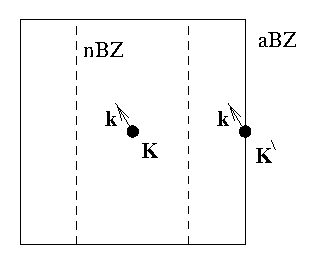
\includegraphics{2d_bz.2.eps}
\end{figure}
%


%%%
%%% Vollst"andigkeit und Orthogonalit"at der \basis 
%%%

Die Funktionen $\basis(\vec{r})$ stellen eine geeignete Basis dar,
da sie vollst"andig und orthonormal sind.

Um die Vollst"andigkeit zu zeigen, verwenden wir, da"s die Bloch-Zust"ande
(\ref{eq:bloch}) eine vollst"andige Basis bilden, d.~h.\ jede Funktion
$f(\vec{r})$ kann nach  Bloch-Zust"anden entwickelt werden 
%
\begin{eqnarray*}
  f(\vec{r}) & = & \sum_{n} \bzint{aBZ} \vdx{\akb} 
        g_{n}(\ak) e^{i\sprod{\ak}{r}} u_{n\ak}(\vec{r}) \\
  & = & \sum_{\set \,n} \: \bzint{nBZ} \vdx{\nkb}
  \underbrace{g_{n}(\nk+\set)}_{\Ts =: g_{n}^{\set}(\nk)} 
  e^{i\sprod{\nk}{r}} \underbrace{e^{i\sprod{\set}{r}}
  u_{n\vec{\nk+\set}}(\vec{r})}_{\mbox{periodisch in nEZ}}.
\end{eqnarray*}
%
Da die beiden letzten Terme periodisch in nEZ sind, k"onnen wir sie nach den
periodischen Funktionen $e^{i\sprod{\set}{r}} u_{n\vec{\set}}$
entwickeln
%
\begin{displaymath}
  e^{i\sprod{\set}{r}} u_{n \nk+\set} = \sum_{\pri{\set}\,\pri{n}}
  b^{\set \pri{\set}}_{n \pri{n}} \! (\nk) \,
  e^{i\sprod{\pri{\set}}{r}} u_{\pri{n} \vec{\pri{\set}}} ,
\end{displaymath}
%
mit den Entwicklungskoeffizienten $b^{\set \pri{\set}}_{n \pri{n}} \! (\nk)$. 
Damit ergibt sich:
%
\begin{displaymath}
  f(\vec{r}) = \sum_{\set \,n} \: \bzint{nBZ} \vdx{\nkb}
  \tilde{g}_{n}^{\set}(\nk) \basis 
  \qquad \mbox{mit} \quad
  \tilde{g}_{n}^{\set}(\nk) = \sum_{\pri{\set}\,\pri{n}}
  b^{\pri{\set} \set}_{\pri{n} n} \! (\nk) \,
  g_{\pri{n}}^{\pri{\set}}(\nk) 
\end{displaymath}
%
Wir sind also in der Lage jede beliebige Funktion $f(\vec{r})$ nach den
Basisfunktionen \basis\ zu entwickeln, was bedeutet, da"s diese vollst"andig
sind. 

Als n"achstes wollen wir die Orthonormalit"at der Basisfunktionen \basis\
zeigen, die durch die folgende Relation ausgedr"uckt wird:
%
\begin{equation}
  \label{eq:orth1}
  \bzint{Kristall}\!\!\!\! \vdx{r} \cc{{\basis}} \pbasis =
  \kronecker{\set}{\pri{\set}} \kronecker{n}{\pri{n}}
  \delta(\nk-\pri{\nk}) 
\end{equation}
%
Da"s dies erf"ullt ist, zeigt sich folgenderma"sen:
%
\begin{eqnarray}
  \label{eq:orth2}
  \bzint{Kristall}\!\!\!\! \vdx{r} \cc{{\basis}}\pbasis & = & 
  \bzint{Kristall}\!\!\!\! \vdx{r} e^{i\sprod{(\pri{k}-k)}{r}}
  \underbrace{e^{i\sprod{(\pri{\set}-\set)}{r}}
  \cc{u_{n\set}}u_{\pri{n}\pri{\set}}}_{\mbox{periodisch in nEZ}} \nonumber \\
  &=& (2\pi)^{3} \sum_{m} \BnnKK{m} \delta(\pri{\nk}-\nk-\nG) \nonumber \\
  &=& (2\pi)^{3} \BnnKK{0} \delta(\vec{\nk}-\nk)
\end{eqnarray}
%
Der letzte Schritt ist richtig, da \nk\ und \pri{\nk} aus der neuen
Brillouin-Zone sind, die durch die \{\nG\} definiert ist. Dabei haben wir eine
Fourier-Trans"-for"-mation durchgef"uhrt
%
\begin{equation}
  \label{eq:bloch-Gm}
  e^{i\sprod{(\pri{\set}-\set)}{r}} \cc{u_{n\set}}u_{\pri{n}\pri{\set}} = 
  \sum_{m} \BnnKK{m} e^{-i\sprod{\nG}{r}}
\end{equation}
%
deren Koeffizienten \BnnKK{m} durch
%
\begin{displaymath}
%  \label{eq:BnnKKm}
  \BnnKK{m} = \frac{1}{\Omega} \bzint{nEZ} \vdx{r}
  e^{i\sprod{\nG}{r}} e^{i\sprod{(\pri{\set}-\set)}{r}}
  \cc{u_{n\set}}u_{\pri{n}\pri{\set}} 
\end{displaymath}
%
gegeben sind, wenn $\Omega$ das Volumen der neuen Einheitszelle ist.
F"ur den Spezialfall $m=0$ gilt
%
\begin{equation}
  \label{eq:BnnKK0}
  \BnnKK{0} = \frac{1}{\Omega} \bzint{nEZ} \vdx{r}
  e^{i\sprod{(\pri{\set}-\set)}{r}} \cc{u_{n\set}}u_{\pri{n}\pri{\set}} =
  \frac{1}{(2\pi)^{3}} \kronecker{\set}{\pri{\set}}
  \kronecker{n}{\pri{n}}
\end{equation}
%
so da"s insgesamt Gl.~\eqref{eq:orth1} erf"ullt ist.

Gl.~\eqref{eq:BnnKK0} ist ein Spezialfall von
%
\begin{equation}
  \label{eq:K.period}
  \bzint{nEZ}e^{i\sprod{k}{r}}f(\vec{r})\vdx{r}=0
\end{equation}
%
f"ur Funktionen $f(\vec{r})$, die periodisch auf aEZ sind, und
$e^{i\sprod{k}{r}}$ periodisch auf nEZ aber nicht auf aEZ, d.~h.\  wenn
$\vec{k} \notin \{\aG\}$ gilt. 
Dies wiederum ist nur ein Spezialfall der allgemeinen Aussage, da"s
%
\begin{displaymath}
  \bzint{Kristall}e^{i\sprod{k}{r}}f(\vec{r})\vdx{r}=0 
\end{displaymath}
f"ur gitterperiodische Funktionen $f(\vec{r})$, wenn $\vec{k}$ kein reziproker
Gittervektor ist.

%%%%%%%%%%%%%%%%%%%%%%%%%%%%%%%%%%%%%%%%%%%%%%%%%%%%%%%%%%%%%%%%%%%%%%%
%%%
%%% Ansatz f"ur die Wellenfunktion
%%%
\section{Ansatz f"ur die Wellenfunktion}
\label{sec:ansatz}

Nachdem gezeigt wurde, da"s unsere Basisfunktionen \basis\ eine geeignete
Basis f"ur die Entwicklung der Eigenfunktionen 
$\psi$ in Gl.~\eqref{eq:h0+h1} sind, soll nun der Ansatz gemacht werden:
%
\begin{displaymath}
%  \label{eq:ansatz}
  \psi = \sum_{\pri{\set},\pri{n}} \bzint{nBZ} \vdx{\pri{\nkb}} \pkoeff
  \pbasis .
\end{displaymath}
%
Wenn wir dies in Gl.~\eqref{eq:h0+h1} einsetzen, so ergibt sich
%
\begin{equation}
  \label{eq:pre-SG}
  \sum_{\pri{\set},\pri{n}} \bzint{nBZ} \vdx{\pri{\nkb}}
  \matrixel{\varbasis}{\op{H_{0}}+\op{H_{1}}}{\pvarbasis} \pkoeff = E \koeff .
\end{equation}
%
Dabei steht \matrixel{\varbasis}{\op{H_{0}}+\op{H_{1}}}{\pvarbasis} f"ur
Matrixelemente bez"uglich der Basisfunktionen $\basis(\vec{r}) =
\braket{\vec{r}}{\varbasis}$. 

%%%%%%%%%%%%%%%%%%%%%%%%%%%%%%%%%%%%%
%%% Matrixelemente von $\op{H_0}$
\subsection{Matrixelemente von \op{H_0}}
\label{sec:h0}

Zun"achst sollen die Matrixelemente von \op{H_{0}} bez"uglich der
Basisfunktionen \basis\ untersucht werden.
%
\begin{equationarray*}{l}
  \matrixel{\varbasis}{\op{H_{0}}}{\pvarbasis}\\
%%%
  \;\; =\bzint{Kristall}\!\!\!\! \vdx{r} e^{-i\sprod{(\nk+\set)}{r}}
  \cc{u_{n\set}} \op{H_{0}} e^{i\sprod{(\pri{\nk}+\pri{\set})}{r}}
  u_{\pri{n}\pri{\set}}\\%[1.3ex]
%%%
  \;\; =\bzint{Kristall}\!\!\!\! \vdx{r} e^{i\sprod{(\pri{\nk}-\nk)}{r}}
  e^{-i\sprod{\set}{r}} \cc{u_{n\set}} 
  (\op{H_{0}} + \frac{\hbar^{2}}{2m} {\pri{\nkb}}^{2} 
  + \frac{\hbar}{m}\sprod{\pri{\nk}}{\op{p}}) e^{i\sprod{\pri{\set}}{r}}
  u_{\pri{n}\pri{\set}}\\%[1.3ex]
%%%
  \;\; =\bzint{Kristall}\!\!\!\! \vdx{r} e^{i\sprod{(\pri{\nk}-\nk)}{r}}
  \underbrace{e^{-i\sprod{\set}{r}} \cc{u_{n\set}} \left(
  \veps_{\pri{n}}(\pri{\set}) + \frac{\hbar^{2}}{2m} {\pri{\nkb}}^{2} +
  \frac{\hbar}{m} \sprod{\pri{\nk}}{\op{p}} \right)
  e^{i\sprod{\pri{\set}}{r}} u_{\pri{n}\pri{\set}}}_{\mbox{periodisch in nEZ}}.
\end{equationarray*}
%
Auf Grund der Periodizit"at in nEZ k"onnen wir "ahnlich wie beim Schritt von
Gl.~\eqref{eq:orth1} zu Gl.~\eqref{eq:orth2} vorgehen. Damit erhalten wir:
%
\begin{equationarray}{l}
\label{eq:preh0}
  \matrixel{\varbasis}{\op{H_{0}}}{\pvarbasis} \nonumber \\[1.5ex]
%%%%
  \;\; =\: \delta(\pri{\nk}-\nk) {\frac{(2\pi)}{\Omega}}^{3} \!\!\!
  \bzint{nEZ}\! \vdx{r} e^{-i\sprod{\set}{r}} \cc{u_{n\set}}
  \left( \veps_{\pri{n}}(\pri{\set}) + \frac{\hbar^{2}}{2m} {\nkb}^{2} +
  \frac{\hbar}{m} \sprod{\nk}{\op{p}} \right) 
  e^{i\sprod{\pri{\set}}{r}} u_{\pri{n}\pri{\set}} \nonumber \\%[1.3ex]
%%%%
  \;\; =\: \delta(\pri{\nk}-\nk) \bigg[ \kronecker{n}{\pri{n}}
  \kronecker{\set}{\pri{\set}} \left( \veps_{n}(\set) 
    + \frac{\hbar^{2}}{2m} \nkb^{2} \right) \nonumber \\%[1.3ex]
%%%%
  \qquad + \: {\frac{(2\pi)}{\Omega}}^{3} \frac{\hbar}{m}
  \bzint{nEZ} \vdx{r} 
  e^{-i\sprod{\set}{r}} \cc{u_{n\set}}  \sprod{\nk}{\op{p}}  
  e^{i\sprod{\pri{\set}}{r}} u_{\pri{n}\pri{\set}}   \bigg] 
\end{equationarray}
%
Der zweite Summand in Gl.~\eqref{eq:preh0} ergibt
%
\begin{equationarray*}{l}
  {\frac{(2\pi)}{\Omega}}^{3} \frac{\hbar}{m} \bzint{nEZ} \vdx{r}
  e^{-i\sprod{\set}{r}} \cc{u_{n\set}} \sprod{\nk}{\op{p}}  
  e^{i\sprod{\pri{\set}}{r}} u_{\pri{n}\pri{\set}} \\
%%%%
  \quad =\: \kronecker{n}{\pri{n}} \kronecker{\set}{\pri{\set}}
  \frac{\hbar}{m} \sprod{\nk}{\set} + {\frac{(2\pi)}{\Omega}}^{3}
  \frac{\hbar}{m} \bzint{nEZ} \vdx{r} e^{i\sprod{(\pri{\set}-\set)}{r}}
  \underbrace{\cc{u_{n\set}} \sprod{\nk}{\op{p}}
  u_{\pri{n}\pri{\set}}}_{\mbox{periodisch in  aEZ}}\\
%%%%
  \quad =\: \kronecker{\set}{\pri{\set}} \frac{\hbar}{m} 
  \left( \kronecker{n}{\pri{n}} \sprod{\nk}{\set} +
  {\frac{(2\pi)}{\Omega}}^{3} \bzint{nEZ}  
  \vdx{r}  \cc{u_{n\set}} \sprod{\nk}{\op{p}} u_{\pri{n}\set} \right) ,
\end{equationarray*}
%
wobei im letzten Schritt Gl.~\eqref{eq:K.period} angewendet wurde.

Es ergeben sich also keine Impulsmatrixelemente zwischen Zust"anden
verschiedener Entwicklungspunkte {\set}. In Anologie zu Gl.~\eqref{eq:pnn}
definieren wir nun:
%
\begin{equation}
  \label{eq:pnnK}
  \pnnK := {\frac{(2\pi)}{\Omega}}^{3} \bzint{nEZ} \vdx{r}
  e^{-i\sprod{\set}{r}} \cc{u_{n\set}} \, \op{\vec{p}}  \,
  e^{i\sprod{\set}{r}} u_{\pri{n}\set}
\end{equation}
%
Damit ergibt sich aus Gl.~\eqref{eq:preh0}:
%
\begin{equation}
  \label{eq:h0}
  \matrixel{\varbasis}{\op{H_{0}}}{\pvarbasis} 
  = \delta(\pri{\nk}-\nk) \kronecker{\set}{\pri{\set}} \left[
  \kronecker{n}{\pri{n}} \left( \veps_{n}(\set) + \frac{k^{2}}{2m}
  \right) + \frac{\sprod{k}{\pnnK}}{m} \right]
\end{equation}
%
Dies entspricht (nat"urlich) dem Ergebnis, das wir in Standard \kdotp-Theorie
f"ur den Punkt \set\ erhalten w"urden, wenn wir uns nur auf einen
Entwicklungspunkt im reziproken Raum beschr"ankt h"atten. Aus
Gl.~\eqref{eq:h0} l"a"st sich also direkt Gl.~\eqref{eq:standard-k.p} ableiten.
Dabei ist nicht nur die Form der Gleichung die selbe, sondern
auch die auftretenden Impulsmatrixelemente sind identisch, da das gr"o"sere
Normierungsvolumen $\Omega$ den Effekt des gr"o"seren Integrationsbereichs nEZ
wieder aufhebt.


%%%%%%%%%%%%%%%%%%%%%%%%%%%%%%%%%%%%%%%%
%%% Matrixelemente von \op{H_1}
\subsection{Matrixelemente von \op{H_1}}
\label{sec:h1}

Die Matrixelemente des St"orpotentials \op{H_{1}} bez"uglich der
Basisfunktionen \basis\ ergeben sich folgenderma"sen:
%
\begin{equation}
  \label{eq:h1mat}
  \matrixel{\varbasis}{\op{H_{1}}}{\pvarbasis} = 
  \bzint{Kristall}\!\!\!\! \vdx{r} e^{-i\sprod{(\nk+\set)}{r}}
  \cc{u_{n\set}} \op{H_{1}} e^{i\sprod{(\pri{\nk}+\pri{\set})}{r}}
  u_{\pri{n}\pri{\set}}
\end{equation}
%
Da \op{H_{1}} ein Potential und damit multiplikativ ist, vertauscht es mit
allen "ubrigen Faktoren innerhalb des Integrals \eqref{eq:h1mat}. Dadurch
ergibt sich der 
gleiche Faktor wie auf der linken Seite von Gl.~\eqref{eq:bloch-Gm}, so da"s
Gl.~\eqref{eq:h1mat} sich mit der Fourier-Entwicklung \eqref{eq:h1-Gm} als
%
\begin{eqnarray*}
%  \label{eq:preh1}
  \matrixel{\varbasis}{\op{H_{1}}}{\pvarbasis} 
  &=&  \sum_{m,\pri{m}} \BnnKK{m} \rho_{\pri{m}} 
  \bzint{Kristall}\!\!\!\! \vdx{r} e^{i\sprod{(\pri{\nk}-\nk)}{r}}
  e^{i\sprod{(\pnG-\nG)}{r}} \nonumber \\
  &=& (2\pi)^{3} \sum_{m,\pri{m}} \BnnKK{m} \rho_{\pri{m}} 
  \delta(\pnG - \pnG + \pri{\nk} - \nk) \nonumber \\
  &=& (2\pi)^{3}  \delta(\pri{\nk} - \nk) 
  \sum_{m,\pri{m}} \BnnKK{m} \rho_{\pri{m}} \kronecker{m}{\pri{m}}
\end{eqnarray*}
%
schreiben l"a"st. Der letzte Schritt ist m"oglich, da \nk\ und
\pri{\nk} aus nBZ sind, zu der die $\{\nG\}$ als reziproke
Gittervektoren geh"oren.
Hier bietet es sich an
%
\begin{eqnarray}
  \label{eq:VnnKK}
  \VnnKK &:=&  (2\pi)^{3} \sum_{m,\pri{m}} \BnnKK{m} \rho_{\pri{m}}
  \kronecker{m}{\pri{m}} \nonumber \\
  &=& {\frac{(2\pi)}{\Omega}}^{3} \bzint{nEZ} \vdx{r}
  e^{-i\sprod{\set}{r}} \cc{u_{n\set}} \op{H_{1}}  
  e^{i\sprod{\pri{\set}}{r}} u_{\pri{n}\pri{\set}}
\end{eqnarray}
%
zu definieren, so da"s wir insgesamt
%
\begin{equation}
  \label{eq:h1}
  \matrixel{\varbasis}{\op{H_{1}}}{\pvarbasis} = 
  \delta(\pri{\nk}-\nk) \VnnKK
\end{equation}
%
erhalten.

Setzen wir nun Gln.~\eqref{eq:h0} und \eqref{eq:h1} in Gl.~\eqref{eq:pre-SG}
ein, so erhalten wir als letztendlich zu l"osende Gleichung:
%
\begin{eqnarray}
  \label{eq:SG}
  \left( \veps_{n}(\set) + \frac{\hbar^{2}}{2m} \nkb^{2} \right) \koeff &+& 
  \frac{\hbar}{m} \sum_{\pri{n}} \sprod{\nk}{\pnnK} A^{\set}_{\pri{n}} \!
  (\nk) \,  \nonumber \\
%%%%
  &+& \sum_{\pri{n},\pri{\set}}  \VnnKK A^{\pri{\set}}_{\pri{n}} \!
  (\nk) \,  = E(\nk) \koeff
\end{eqnarray}
%

Es ist auffallend, da"s Gl.~\eqref{eq:SG} diagonal in \nk\ ist, weshalb sich
die Energieeigenwerte $E(\nk)$ wieder nach dem Kristallimpuls \nk\ 
klassifizieren lassen, d.~h.\ es ergibt sich wiederum eine Bandstruktur. Dies
unterscheidet sich von dem, was Luttinger und Kohn \cite{luko:55} bei der
Ableitung der EFA erhielten, die dieser Herleitung als Vorbild diente. Doch
ist dies einfach dadurch zu erkl"aren, da"s hier von einer periodischen
St"orung \eqref{eq:K.period} ausgegangen wurde und damit -- bei geeigneter
Wahl der Entwicklungspunkte im reziproken Raum -- auch ihre Matrixelemente
diagonal in \nk\ sind.\footnote{Die hier gezeigt Ableitung ist so allgemein
  gehalten, da"s sie auch f"ur nicht strengperiodische St"orungen anwendbar
  ist. So z.~B.\ St"orungen mit periodisch angeordneten Gau"s-Funktionen
  anstelle der Deltafunktionen als Fourier-Transformierte.}

%%%%%%%%%%%%%%%%%%%%%%%%%%%%%%%%%%%%%%%%%%%%%%%%%%%%%%%%%%%%%%%%%%%
%%%
%%% Diskussion
%%%
\section{Diskussion}
\label{sec:disk}

Als erstes ist festzustellen, da"s sich Gl.~\eqref{eq:SG} auf die
normale \kdotp-Gleichung \eqref{eq:standard-k.p} reduziert, wenn alle \VnnKK\ 
verschwinden und nur ein Entwicklungspunkt \set\ herangezogen wird. Schreiben
wir Gl.~\eqref{eq:SG} f"ur nichtverschwindende \VnnKK\ und zwei
Entwicklungspunkte in Matrixform, so erhalten wir eine Matrix der Form

\begin{displaymath}
\left(
  \begin{array}{c|c}
    \begin{minipage}[t][\Matrixform][c]{\Matrixform}
      \begin{center}
        Standard \kdotp-Matrix f"ur\\
        \set\ als Entwicklungspunkt + \VnnKKee
      \end{center}
    \end{minipage}&
    \begin{minipage}[t][\Matrixform][c]{\Matrixform}
      \begin{center}
        \VnnKK
      \end{center}
    \end{minipage}\\
    \hline
    \begin{minipage}[t][\Matrixform][c]{\Matrixform}
      \begin{center}
        \VnnKKze
      \end{center}
    \end{minipage}&
    \begin{minipage}[t][\Matrixform][c]{\Matrixform}
      \begin{center}
        Standard \kdotp-Matrix f"ur\\ 
        \pri\set\ als Entwicklungspunkt + \VnnKKzz
      \end{center}
    \end{minipage}
  \end{array}
\right)
\end{displaymath}
%
f"ur den Hamilton-Operator $\op{H_{0}}+\op{H_{1}}$ in der Basis der \basis.
Dabei stellt jeder der obigen Quadranten eine unendlich-dimensionale Matrix
dar, da es zu jedem Punkt im reziproken Raum unendlich viele L"osungen der
ungest"orten Schr"odingergleichung \eqref{eq:ungestoert} gibt, und damit auch
unendlich viele Basisfunktionen \basis\ zu jedem Entwicklungspunkt \set.

Insgesamt ist es also gelungen, die Differentialgleichung \eqref{eq:h0+h1} auf
die algebraische Gleichung \eqref{eq:SG} zur"uckzuf"uhren. Da hierf"ur ein
vollst"andiges Orthonormalsystem von Zust"anden verwendet wurde, ist
Gl.~\eqref{eq:SG} "aquivalent zu Gl.~\eqref{eq:h0+h1}. Dies ist vergleichbar
zu der in Kap.~\ref{sec:standard-k.p} gezeigten Situation in normaler
\kdotp-Theorie, wo auch ein differentielles Problem auf ein
unendlich-dimensionales algebraisches Problem zur"uckgef"uhrt wird
\cite{kane:66}.  Dieses unendlich dimensionale Problem k"onnen wir wieder mit
Hilfe der L"owdin-St"orungstheorie auf ein endlich-dimensionales Problem
reduzieren, wenn wir die Basisfunktionen \basis\ in zwei Gruppen zerlegen
k"onnen, wie in Kap.~\ref{sec:standard-k.p} skizziert.

%%%%%%%%%%%%%%%%%%%%%%%%%%%%%%%%%%%%
\subsection{M"ogliche Erweiterungen}
\label{sec:erweiterungen}

Da Gl.~\eqref{eq:SG} formal gro"se "Ahnlichkeit mit der Standard
\kdotp-Gleichung \eqref{eq:standard-k.p} aufweist, sind die in
Kap.~\ref{sec:standard-k.p} erw"ahnten Erweiterungen auch hier m"oglich.

So ist es sinnvoll, die Spin-Bahn-Wechselwirkung \eqref{eq:Spin-Bahn} als
zus"atzlichen Term im Hamilton-Operator zu ber"ucksichtigen, wenn die
Dispersion im Valenzband beschrieben weden soll. Es bietet sich an, diesen
Term wiederum st"orungstheoretisch zu behandeln, da sich dann die Anzahl der
notwendigen Impulsmatrixelemente \pnnK\ und Potentialmatrixelemente \VnnKK\ 
nicht erh"oht.  F"ur die Wechselwirkung mit anderen Zust"anden m"ussen wir
analog zu Kap.~\ref{sec:standard-k.p} von \pnnK\ zu
$\grvec{\pi}^{\set}_{\mathnormal{n\pri{n}}}$ "ubergehen, die sich in ihrer
Definition darin unterscheiden, da"s in Gl.~\eqref{eq:pnnK} \vecop{p} durch
$\vecop{p} + \frac{\hbar}{4mc^{2}} (\grvecop{\sigma} \times \nabla\op{V})$
ersetzt werden mu"s \cite{luko:55}.

Da in Gl.~\eqref{eq:Spin-Bahn} der Gradient des Kristallpotentials \op{V}
auftritt, stellt sich die Frage, ob das St"orpotential \op{H_{1}} hier
ber"ucksichtigt werden mu"s. Normalerweise ist dies nicht zu erwarten, da die
Spin-Bahn-Wechselwirkung auf Grund des St"orpotential \op{H_{1}} eine St"orung
h"oherer Ordnung darstellt. Falls die St"orung \op{H_{1}} aber (teilweise)
durch Relaxationen hervorgerufen wird, so ist es vorstellbar, da"s \op{H_{1}}
zwar klein ist, die Gradienten von \op{H_{1}} aber vergleichbar zu denen des
Kristallpotentials sind.

Weiterhin k"onnen auch die Methoden von Bir und Pikus \cite{bipi:74} zur
Ber"ucksichtigung von Verzerrungen durch externen Druck im Rahmen unserer
Theorie angewendet werden. Auch der Schritt von Standard \kdotp-Theorie zur
EFA l"a"st sich verallgemeinern, so da"s auch der Einflu"s flacher St"orstellen
oder Magnetfelder untersucht werden kann. Dabei k"onnen wir dem Vorgehen von
Luttinger und Kohn \cite{luko:55} folgen, da die von uns gew"ahlte Basis
\eqref{eq:basis} sehr "ahnlich zu der Basis ist, die sie verwendeten. F"ur
St"orstellen k"onnte es dabei m"oglich sein, nicht"aquivalente Einbaupl"atze
zu unterscheiden.

%%%%%%%%%%%%%%%%%%%%%%%%%%%%%%%%%%%%%%%%%%%%
\subsection{Vergleich mit anderen Methoden}
\label{sec:vergleich}

Eine "ahnliche Methode zur Ber"ucksichtigung der Mischung von Zust"anden von
verschiedenen Punkten des reziproken Raumes im Rahmen von \kdotp\ bzw.\ EFA
hat Foreman \cite{fore:98-2} vorgeschlagen. Er geht dabei unmittelbar von
einer gr"o"seren Einheitszelle aus, die der hier verwendeten nEZ entspricht.
Bez"uglich der mit dieser Einheitszelle verbundenen Brillouin-Zone geh"oren
alle Blochzust"ande, die hier zur Basis beitragen, zu \emph{einem} Punkt des
reziproken Raumes. Damit entf"allt der in Kap.~\ref{sec:basis} gef"uhrte
Beweis der Vollst"andigkeit und Orthonormalit"at und normale
\kdotp-Gleichungen k"onnen f"ur das ungest"orte Problem verwendet werden. F"ur
die durch das St"orpotential induzierten Wechselwirkungen -- bei Foreman das
Potential eines einzelnen Hetero"ubergangs zwischen AlAs und GaAs -- ergeben
sich dann Matrixelemente zwischen Blochzust"anden an \emph{einem} Punkt des
reziproken Gitters. 

Dieser Ansatz ist im wesentlichen "aquivalent zu dem hier
gew"ahlten.  Allerdings geht die Blockdiagonal-Form des Hamilton-Operators
bez"uglich der \kdotp-Wechselwirkung zun"achst verloren. Der
\kdotp-Hamilton-Operator f"ur die gr"o"sere Einheitszelle enth"alt zun"achst
Impulsmatrixelemente, deren Verschwinden erst aus einer zus"atzlichen
Betrachtung folgt. Vergleichbar zu den hier erhaltenen Ergebnissen w"urde sich
bei einer solchen Betrachtung auch ergeben, da"s die tats"achlich ben"otigten
Impulsmatrixelemente die gleichen sind, wie sie in einer \kdotp-Rechnung f"ur
den ungest"orten Kristalls in seiner primitiven Einheitszelle ben"otigt
werden, wenn alle \{\set\} unabh"angig voneinander als Entwicklungspunkte
verwendet werden. Dies ist deshalb von Vorteil, da der ungest"orte Kristall im
Allgemeinen eine h"ohere Symmetrie aufweist, so da"s aus gruppentheoretischen
Gr"unden insgesamt weniger unabh"angige Parameter zu ber"ucksichtigen sind.

Bei dem Problem der Mischung von Blochzust"anden wie es Foreman betrachtet,
spielt dies nur eine untergeordnete Rolle. Doch hier sollen auch
Energiedispersionen berechnet werden, und da ist diese Reduzierung der Anzahl
der unabh"angigen Paramter wichtig. 

Das f"ur die Berechnung der Energiedispersionen verwendete Verfahren weist
"Ahnlichkeiten mit Methoden auf, die auf Cardona zur"uckgehen \cite{card:63}.
Dabei werden die Impulsmatrixelemente in Halbleitern mit Zinkblende-Gitter auf
entsprechenden Matrixelemente isoelektrischer Halbleiter mit Diamant-Gitter
zur"uckgef"uhrt.\footnote{D.~h.  da"s z.~B.\ Impulsmatrixelemente f"ur GaAs
  auf die in Ge zur"uckgef"uhrt werden.}  Das inversions-asymmetrische
Potential, das den Unterschied zwischen Zinkblende- und Diamant-Struktur
beschreibt, wird dazu als St"orung eines zugrundeliegenden Diamant-Gitters
aufgefa"st.  Die Blochzust"ande der polaren Materialien k"onnen dadurch als
"Uberlagerung von Zu"-st"an"-den eines unpolaren Materials dargestellt werden.
Damit ergeben sich auch die Impulsmatrixelemente aus "Uberlagerungen der
Impulsmatrixelemente des unpolaren Materials. Im Diamant-Gitter gibt es aber
auf Grund der h"oheren Symmetrie weniger unabh"angige Parameter, so da"s auf
diesem Weg unbekannte Impulsmatrixelemente der Zinkblende-Struktur durch
bekannte Energieunterschiede und Impulsmatrixelemente des isoelektrischen
Diamant-Gitters ausgedr"uckt werden k"onnen. Der wesentliche Unterschied zu
dem hier behandelten Problem besteht darin, da"s das von Cardona verwendete
St"orpotential das Bravais-Gitter des Kristalls nicht "andert, so da"s keine
Mischung von Zust"anden verschiedener Punkte im \vec{k}-Raum auftritt. 
Zudem ist es in diesem Fall ausreichend, nur \emph{ein} Impulsmatrixelement und
\emph{ein} Potentialmatrixelement zu ber"ucksichtigen, was das Problem
deutlich vereinfacht.


%. Dadurch sind keine
%relativen Phasen zu beachtet, was nicht immer einfach ist, wie wir in
%Kap.~\ref{sec:phase} sehen werden. Wie dieses Problem sowie die nicht-triviale
%Bestimmung der \VnnKK behandelt werden kann, soll nun im n"achsten Kapitel
%gezeigt werden.

%%% local Variables: 
%%% mode: latex
%%% TeX-master: "diplom"
%%% End: 

